% ============================================================================
% AuditIQ -- phase-1 project paper
% Layout follows the first draft: Introduction, Related Work, (Base Papers),
% Proposed Methodology, System Implementation, Experimental Setup,
% (Expected) Results and Discussion, Explainability, Limitations, Future Work,
% Conclusion, Data and Code Availability.
%
% Compile:  pdflatex auditiq_paper.tex   (run twice; needs fig_architecture.pdf)
% Figure:   python make_figure.py        (regenerates fig_architecture.pdf)
%
% BEFORE SENDING THIS TO AN EXTERNAL VENUE
%  1. Run the protocol of Section VI and replace Section VII with measured
%     results. This draft reports no performance numbers for AuditIQ, because
%     none have been measured yet.
%  2. Section III and Table I were written from the abstracts of the three
%     base papers. Read the full papers and correct anything they contradict.
%  3. Section V names the LLM only as "an open-weight LLM". Replace it with the
%     exact model identifier and version used in the runs.
%  4. The reference to Roumeliotis et al. is copied from the earlier draft; its
%     DOI resolves, but confirm title, volume and pages on IEEE Xplore.
% ============================================================================
\documentclass[conference]{IEEEtran}
\IEEEoverridecommandlockouts
% T1 encoding makes XeTeX-based engines (e.g. Tectonic) use the same Times
% fonts as pdfLaTeX; without it they fall back to Latin Modern with no bold
% or italics.
\usepackage[T1]{fontenc}
\usepackage{cite}
\usepackage{amsmath,amssymb}
\usepackage{graphicx}
\usepackage{booktabs}
\usepackage{array}
\usepackage{url}

\newcolumntype{L}[1]{>{\raggedright\arraybackslash}p{#1}}

\begin{document}

\title{AuditIQ: A Controls-First Multi-Agent Framework with Evidence-Grounded Confidence Weighting for Explainable Procurement Audit}

\author{\IEEEauthorblockN{Podichetty Samiksha}
\IEEEauthorblockA{\textit{Department of Information Technology} \\
\textit{Chaitanya Bharathi Institute of Technology}\\
Hyderabad, Telangana, India \\
samiksha10.1b@gmail.com}
\and
\IEEEauthorblockN{Chandana Devanaboyina}
\IEEEauthorblockA{\textit{Department of Information Technology} \\
\textit{Chaitanya Bharathi Institute of Technology}\\
Hyderabad, Telangana, India \\
chandanad3884@gmail.com}
}

\maketitle

\begin{abstract}
Auditing procurement transactions means matching every invoice against its purchase order, goods receipt, vendor record and approval trail, and justifying each exception against a written policy. The base papers of this work leave three gaps: an anomaly detector returns a label without the violated rule; large language models (LLMs) explain the errors they find poorly and rarely cite the governing standard; and a multi-agent recommender does not use the reliability signal that agreement between its agents provides. This paper presents AuditIQ, a multi-agent pipeline for the procure-to-pay process that reads the active policy at run time, has a challenger agent remove unsupported findings, and routes high-risk transactions to a human reviewer. We extend the working prototype with five features: deterministic controls that run before any LLM; an evidence-grounded confidence for every finding; a confidence-weighted risk score with a sampled-review queue, which provably never changes which transactions are auto-approved; clause-level policy parameters; and AuditIQ-Bench, a synthetic benchmark with fourteen labelled anomaly classes. The paper gives the technology stack and implementation status of every feature and an evaluation protocol with six configurations. Expected results are stated as hypotheses with the observation that would refute each; measured results will follow the experimental runs.
\end{abstract}

\begin{IEEEkeywords}
audit analytics, multi-agent systems, large language models, procure-to-pay, three-way matching, explainable AI, human-in-the-loop, confidence weighting
\end{IEEEkeywords}

\section{Introduction}
An auditor who tests procurement spend has to establish four things for every invoice: that it corresponds to an approved purchase order (PO), that the goods or services were received as recorded in a goods receipt note (GRN), that the vendor is legitimate and tax-compliant, and that the payment was approved within the approver's delegated limit. The evidence for these checks sits in separate records, and the definition of an exception is written in an organization-specific policy document. Because the work is repetitive, it is usually performed on a sample~\cite{elder2013}, which leaves most of the population untested. Continuous auditing proposes to test every transaction automatically~\cite{vasarhelyi1991}.

Three recent works approach this goal, and each leaves a gap (Section~\ref{sec:base}). An anomaly detector scores financial records accurately but returns a label~\cite{long2026}, not the violated rule and its evidence, which audit documentation standards require~\cite{isa230}. LLMs explain errors poorly and rarely cite the governing standard~\cite{wang2025auditbench}. A multi-agent recommender shows that agreement between specialist models predicts correctness, yet its combined accuracy does not exceed that of its best single model~\cite{toudas2026}.

This paper presents AuditIQ, a multi-agent pipeline for transaction-level procurement audit built on four principles.
\begin{itemize}
\item \textit{Controls first.} Checks that are decidable by arithmetic or lookup are executed as code, before any LLM is called.
\item \textit{Policy as data.} The active policy document is stored with a version number and read at run time; every finding cites one of its clauses.
\item \textit{Adversarial verification.} A challenger agent reviews all findings and removes those the evidence does not support.
\item \textit{Governed outcomes.} A risk score routes each transaction to automatic approval or to a human reviewer, and every stage writes to an audit trail.
\end{itemize}

AuditIQ exists as a working prototype. This paper describes it, specifies five extra features, fixes their technology stack, and states the expected results in a form that measurement can refute. The main contributions are as follows.
\begin{itemize}
\item A controls-first multi-agent architecture for procure-to-pay audit, with a working prototype.
\item An evidence-grounded confidence for every finding and a confidence-weighted risk score with a sampled-review tier, which provably leaves the set of auto-approved transactions unchanged.
\item A policy store with clause-level parameters, so that a change of policy needs no change to the pipeline.
\item AuditIQ-Bench, a specification for a synthetic procure-to-pay benchmark with fourteen labelled anomaly classes and purpose-built hard negatives.
\item An evaluation protocol with six system configurations, and expected results stated as falsifiable hypotheses.
\end{itemize}

The paper reports no measured performance for AuditIQ. Section~\ref{sec:expected} states expectations, not results.

\section{Related Work}
\subsection{Anomaly Detection in Accounting Data}
Statistical fraud detection has a long history~\cite{bolton2002}, and anomaly detection methods are surveyed in~\cite{chandola2009}. In auditing, digit-distribution tests based on Benford's law remain a standard screening tool~\cite{nigrini2017}. Unsupervised detectors such as isolation forests~\cite{liu2008} and one-class support vector machines~\cite{scholkopf2001} need no labelled fraud cases, and autoencoders have been applied to journal entries at scale~\cite{schreyer2017}. These methods rank records by how unusual they are. An unusual record is not necessarily a policy violation, and a violation, such as an invoice approved above a delegated limit, need not look unusual.

\subsection{Large Language Models in Auditing}
LLMs have been applied to matching passages of financial reports against audit requirements~\cite{hillebrand2023} and to verifying the regulatory compliance of financial reports~\cite{berger2023}. Two known weaknesses of LLMs matter for audit use. Generated text can assert facts that the input does not support~\cite{ji2023}. Grounding the generation in retrieved documents~\cite{lewis2020} and delegating computation to tools~\cite{yao2023} reduce this risk but do not remove it.

\subsection{Multi-Agent Verification and Confidence}
Letting agents criticize one another's answers improves factual accuracy~\cite{du2024}, and sampling a model several times and keeping the majority answer improves reasoning accuracy~\cite{wang2023sc}. Confidence is harder to obtain. Neural classifiers are often over-confident~\cite{guo2017}, and the confidence that an LLM states in words is poorly calibrated~\cite{xiong2024}. Roumeliotis et al.~\cite{roumeliotis2026} use trust scores when orchestrating agents. For high-stakes decisions, human review of uncertain cases is the accepted safeguard~\cite{mosqueira2023,nistrmf}.

\subsection{Research Gap}
No work we know of executes audit controls as code, lets agents add only what code cannot decide, measures how well each finding is supported, and uses that measure to decide what a human must review.

\section{Base Papers}
\label{sec:base}
AuditIQ builds on three recent works. This section states what each does, what it reports, and what it leaves open.

\subsection{Audit Anomaly Detection with an Optimized One-Class SVM}
Long et al.~\cite{long2026} address anomaly detection in the financial auditing of construction projects. They collect 2,400 financial records, comprising statements, invoices and transaction records, normalize the text, and handle missing values. Each record is represented by TF--IDF vectors and Word2Vec embeddings. A one-class support vector machine with adaptive sample weights learns the boundary of normal records, and its parameters are tuned with the Big Bang--Big Crunch metaheuristic. Consistency across validation folds is checked with paired $t$-tests. The reported detection metrics lie between 0.95 and 0.97 and exceed those of conventional machine-learning baselines.

\textit{What it leaves open.} The model scores each record from its text features and returns an anomaly decision. It does not name the violated rule or the supporting evidence, and it learns what is normal from data, so a change of policy requires retraining.

\subsection{AuditBench}
Wang et al.~\cite{wang2025auditbench} ask how well LLMs can audit financial statements. They build a benchmark that pairs real financial tables with synthesized transaction data into which errors are injected, and evaluate models in a five-stage framework that includes mapping each error to the accounting standard it violates. Current LLMs identify errors when given the transaction history, but are markedly weaker at explaining them and at citing the relevant standard, and they struggle to carry out a complete audit.

\textit{What it leaves open.} AuditBench measures models. It does not propose a system that overcomes the weaknesses it finds, and it concerns errors in financial statements, not the matching of procurement documents.

\subsection{Explainable Multi-Agent Recommender}
Toudas et al.~\cite{toudas2026} build an explainable recommender for access control over financial documents. FinBERT, BERT-base-uncased and GPT-4.1-mini are fine-tuned on Financial PhraseBank sentences labelled with four sensitivity levels. A GPT-5.1 orchestrator combines their predictions in zero-shot mode and writes a natural-language justification. The system reaches 83.71\% accuracy, against 82.80--84.93\% for the individual models. When all three models agree, which happens in 78.8\% of cases, accuracy is 92.28\%.

\textit{What it leaves open.} Agreement predicts correctness, but the combined accuracy does not exceed the best single model, so the signal is not yet turned into a better decision. The task is the classification of single sentences, not the audit of linked records.

\subsection{What AuditIQ Adopts}
AuditIQ takes the detector family of Long et al. as a baseline; the injection of labelled errors into synthetic transactions and the measurement of citation quality from AuditBench; and specialist agents with agreement as a reliability signal from Toudas et al., feeding that signal into the risk score. Table~\ref{tab:positioning} summarizes the comparison.

\begin{table*}[t]
\caption{AuditIQ and Its Base Papers}
\label{tab:positioning}
\centering
\footnotesize
\setlength{\tabcolsep}{3pt}
\renewcommand{\arraystretch}{1.12}
\begin{tabular}{L{2.2cm}L{4.0cm}L{3.9cm}L{3.4cm}L{3.5cm}}
\toprule
Work & Task and data & Method & Rule and evidence in the output & Reliability signal \\
\midrule
Long et al.~\cite{long2026} & Anomaly detection over 2,400 construction-industry financial records & TF--IDF and Word2Vec features; optimized adaptive-weighted one-class SVM & Anomaly label & None reported \\
Wang et al.~\cite{wang2025auditbench} & Benchmark of LLMs on financial-statement auditing with synthesized transactions & Single LLM evaluated in five stages & Explanation and standard citation are evaluated and found weak & None reported \\
Toudas et al.~\cite{toudas2026} & Sensitivity classification of financial text into four classes & Three fine-tuned specialists and a zero-shot reasoning orchestrator & Natural-language justification & Agent agreement, analyzed after the decision \\
AuditIQ (this work) & Transaction-level audit of linked invoice, PO, GRN, vendor and approval records & Deterministic controls, three specialist agents, challenger & Finding with policy clause and evidence fields; audit pack & Per-finding confidence from grounding, clause validity and agreement, used in scoring and routing \\
\bottomrule
\end{tabular}
\end{table*}

\section{Proposed Methodology}
\label{sec:method}
\subsection{System Overview}
Fig.~\ref{fig:arch} shows the pipeline. A transaction $x$ is the tuple of records linked to one invoice: the invoice, its PO, its GRN, the vendor master record, and the approval log entries. A policy version $P_v$ is a document whose clauses carry identifiers; $K(P_v)$ denotes its set of clause identifiers. For each transaction the system outputs a set of findings, called flags, $F(x)$; a risk score; a route; and an audit pack. A flag is a tuple
\begin{equation}
f=(k,\,s,\,E,\,\sigma,\,c),
\label{eq:flag}
\end{equation}
where $k\in K(P_v)$ is the cited clause, $s$ is the severity (critical, high, medium or low), $E$ is the set of evidence fields and the values the flag relies on, $\sigma\in\{\mathrm{D},\mathrm{L}\}$ records whether the flag comes from a deterministic control or an LLM agent, and $c\in[0,1]$ is its confidence. The ground truth of $x$ is the set $Y(x)\subseteq K(P_v)$ of clauses it violates; $x$ is clean when $Y(x)=\emptyset$.

\begin{figure*}[t]
\centering
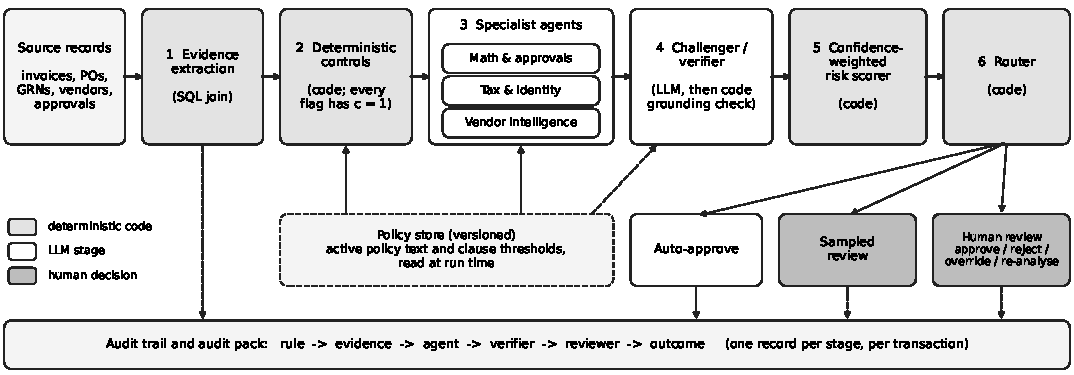
\includegraphics[width=\textwidth]{fig_architecture.pdf}
\caption{AuditIQ pipeline with the extra features. Stages 1, 2, 5 and 6 are deterministic code; stages 3 and 4 use an LLM. The policy store is read at run time by the controls, the agents and the verifier. Every stage appends a record to the audit trail.}
\label{fig:arch}
\end{figure*}

\subsection{Existing Pipeline}
\subsubsection{Evidence extraction}
The input identifier is resolved to a transaction by a single SQL join of the invoice with its PO, GRN and vendor record, so every later stage sees the same values. A vendor identifier yields all of that vendor's invoices, which the pattern checks need.

\subsubsection{Policy store}
Policies are stored as versioned rows that hold the policy text and mark the active version. At the start of each run the active version is read and inserted into every agent prompt, and its version number is written to the result record.

\subsubsection{Specialist agents}
Three LLM agents run in parallel, each with a narrow remit. The \textit{math and approvals} agent examines amounts, quantities and approval limits. The \textit{tax and identity} agent examines duplicate invoices and tax identifiers (GSTIN). The \textit{vendor intelligence} agent examines behavioral patterns in the vendor's history; in production it may also search external sources for adverse information. Each returns a JSON array of flags.

\subsubsection{Challenger}
An LLM challenger receives all flags and is instructed to remove any flag whose evidence does not support it or whose severity is not justified, and to return the kept and the removed flags with reasons.

\subsubsection{Count-based risk score}
A transaction is scored by the severities of its verified flags:
\begin{equation}
R_0(x)=\min\Bigl(100,\ \sum_{f\in F(x)} w_{s(f)}\Bigr),
\label{eq:r0}
\end{equation}
with weights $w=(30,20,10,5)$ for critical, high, medium and low. A floor then raises $R_0$ to at least 70 if $F(x)$ contains a critical flag, and otherwise to at least 50 if it contains a high flag. The transaction is escalated to a human when $R_0(x)\ge\tau$, with $\tau=50$. Every flag counts fully, whether it was computed from database values or inferred by an LLM.

\subsubsection{Human review and audit pack}
An escalated transaction pauses the pipeline. The reviewer sees the risk result, the verified flags and the extracted evidence, and approves, rejects or overrides with a written justification; an analysis can also be sent back for re-analysis. The final stage writes an audit pack (Section~\ref{sec:xai}).

\subsection{Extra Features}
\label{sec:extra}
Five features extend the prototype.

\subsubsection{E1: Controls-first stage}
In the prototype the agents perform the rule checks themselves, with control functions attached as tools. E1 moves every check that is decidable from the extracted values into a separate stage that runs before the agents: matching of amounts and quantities across invoice, PO and GRN, duplicate invoice numbers, GSTIN checks, approval limits, missing documents, blacklist status, and the count, weekday and round-amount indicators (classes R1--R10 in Table~\ref{tab:taxonomy}). Each control is a pure function of the transaction and the policy parameters, and emits a flag with source $\sigma=\mathrm{D}$. The agents then receive the control flags and add only what code cannot decide: a short delivery explained in a GRN remark, invoices structured across days to stay under an approval limit, near-duplicate invoices whose numbers were re-keyed, and invoice descriptions that do not match the PO (classes J1--J4), each with $\sigma=\mathrm{L}$.

\subsubsection{E2: Evidence-grounded confidence}
Each flag receives a confidence
\begin{equation}
c(f)=
\begin{cases}
1, & \sigma(f)=\mathrm{D},\\[2pt]
\tfrac{1}{3}\bigl(g(f)+p(f)+a(f)\bigr), & \sigma(f)=\mathrm{L},
\end{cases}
\label{eq:conf}
\end{equation}
where
\begin{itemize}
\item $g(f)\in\{0,1\}$ is \textit{grounding}: 1 if every field in $E$ exists in the extracted transaction with the stated value;
\item $p(f)\in\{0,1\}$ is \textit{clause validity}: 1 if $k\in K(P_v)$ for the active version;
\item $a(f)\in[0,1]$ is \textit{agreement}: the fraction of $m$ independent re-runs of the originating agent that return a flag citing the same clause for the same transaction.
\end{itemize}
The first two terms are computed by code after the challenger. The third costs $m$ further agent calls and is computed only for transactions that carry at least one LLM flag. None of the terms relies on a confidence stated by the model, which is poorly calibrated~\cite{xiong2024}; agreement is used because it has been observed to predict correctness~\cite{toudas2026,wang2023sc}. Equal weights are an uninformed starting point, and the protocol includes a sensitivity analysis.

\subsubsection{E3: Confidence-weighted score and sampled review}
\label{sec:scoring}
The weighted score is
\begin{equation}
R_c(x)=\min\Bigl(100,\ \sum_{f\in F(x)} w_{s(f)}\,c(f)\Bigr),
\label{eq:rc}
\end{equation}
with the same floors applied only for flags with $c(f)\ge\theta$, where $\theta=2/3$. Routing uses both scores:
\begin{equation}
\mathrm{route}(x)=
\begin{cases}
\text{escalate}, & R_c(x)\ge\tau,\\
\text{sample}, & R_c(x)<\tau\le R_0(x),\\
\text{approve}, & R_0(x)<\tau.
\end{cases}
\label{eq:route}
\end{equation}

Because $c(f)\le 1$, and because the floors of $R_c$ are triggered by a subset of the flags that trigger the floors of $R_0$, we have $R_c(x)\le R_0(x)$ for every $x$. By~\eqref{eq:route}, a transaction is approved exactly when $R_0(x)<\tau$. The set of auto-approved transactions is therefore identical under both scores. Confidence weighting only divides the transactions that the count-based score escalates into two queues: those escalated on well-supported flags, and those escalated only because of weakly supported flags. The latter go to a sampled-review queue, of which a configurable fraction $\rho$ is reviewed by a human. With $\rho=1$ the scheme reduces to the count-based baseline.

\textit{Illustration (constructed, not measured).} A transaction carries a round-amount indicator from a control (medium, $c=1$) and a near-duplicate flag from an agent (critical). The agent's flag cites a matching invoice number that is absent from the extracted data ($g=0$), cites a valid clause ($p=1$), and is reproduced by one of three re-runs ($a=1/3$), so $c=4/9$. The count-based score is $R_0=40$, raised to 70 by the critical floor, and the transaction is escalated. The weighted score is $R_c=10+30\cdot\tfrac{4}{9}\approx 23.3$ with no floor, since $4/9<\theta$. The transaction is routed to sampled review.

\subsubsection{E4: Clause-level policy parameters and deterministic routing}
The numeric thresholds of a policy version, such as the match tolerance, the daily invoice count and the approval limits, are held in a parameter table keyed by clause identifier. The controls read the parameters and the agents read the clause text of the same version, so a change of policy requires no change to the pipeline. The router, which the prototype implements with an LLM, becomes a deterministic condition on~\eqref{eq:route}.

\subsubsection{E5: AuditIQ-Bench and evaluation harness}
A seeded generator produces linked procurement records with labelled anomalies, and a harness runs every configuration against them (Section~\ref{sec:protocol}).

\subsection{Overall System Workflow}
With the extra features in place, a transaction is processed as follows.
\begin{enumerate}
\item An invoice or vendor identifier is submitted, singly or by the batch runner.
\item Evidence extraction joins the linked records into one transaction, and the active policy version and its parameters are read.
\item The deterministic controls run and emit flags with $c=1$.
\item The three specialist agents run in parallel and emit judgement flags.
\item The challenger removes unsupported flags; code computes grounding and clause validity for the rest.
\item For a transaction with LLM flags, the originating agents are re-run $m$ times to obtain agreement, and both scores are computed.
\item The router sends the transaction to automatic approval, sampled review or human review.
\item The audit pack and the per-stage records are written, and any reviewer decision is stored with its justification.
\end{enumerate}

\begin{table}[t]
\caption{Anomaly Classes of AuditIQ-Bench}
\label{tab:taxonomy}
\centering
\footnotesize
\setlength{\tabcolsep}{3pt}
\begin{tabular}{L{0.6cm}L{6.1cm}L{1.3cm}}
\toprule
ID & Anomaly class & Severity \\
\midrule
\multicolumn{3}{l}{\textit{Rule-defined (decidable from field values)}} \\
R1 & Invoice amount differs from PO amount beyond the tolerance & High \\
R2 & Billed quantity exceeds received quantity & High \\
R3 & Duplicate invoice number for the same vendor & Critical \\
R4 & Malformed GSTIN or invalid state code & Medium \\
R5 & Invoice GSTIN differs from the vendor master & High \\
R6 & Same-day invoice splitting above the daily count & High \\
R7 & Invoice amount exceeds the approver's limit & Critical \\
R8 & Missing PO or GRN reference & High \\
R9 & Vendor blacklisted or suspended & Critical \\
R10 & Weekend-dated or round-amount invoice & Low/Med. \\
\addlinespace
\multicolumn{3}{l}{\textit{Judgement (free text or cross-record reasoning)}} \\
J1 & Near-duplicate invoice: re-keyed number, same vendor and amount & Critical \\
J2 & Cross-day structuring just below an approval limit & High \\
J3 & Invoice description inconsistent with the PO description & Medium \\
J4 & GRN remark contradicts the billed quantity & High \\
\bottomrule
\end{tabular}
\end{table}

\section{System Implementation}
\label{sec:impl}
\subsection{Technology Stack}
Table~\ref{tab:stack} gives, for every feature, the technology with which it is or will be built, the reason for the choice, and its status. Three decisions shape the stack.

\textit{Orchestration.} The agent graph runs in Flowise~\cite{flowise}, an open-source visual framework whose Agentflow nodes provide agents, LLM calls, conditions, loops and a human-input step. Each flow is exposed as a REST endpoint, which is all the evaluation harness needs. Self-hosting it with Docker fixes the version used in the experiments.

\textit{Model access.} The agents call the LLM through a LiteLLM gateway~\cite{litellm}, so the model can be replaced without editing the graph. The experiments use one open-weight LLM at temperature 0 and repeat the main comparison with a second model.

\textit{Controls in the database.} The deterministic controls are written as SQL views over the relational store, extended by small JavaScript functions where a view is impractical. The pipeline and the controls-only baseline therefore execute one and the same definition.

\subsection{Current Prototype}
The prototype is an Agentflow graph with three agent nodes, LLM nodes for the challenger and the audit pack, a human-input node, and function nodes for extraction, policy retrieval, aggregation and scoring. Six control functions exist as JavaScript tools: three-way match, duplicate invoice, GSTIN check, approval limit, vendor policy and ledger pattern. The agent prompts repeat some thresholds from the policy; these will be removed so that the policy store is the only source. A batch runner submits pending invoices to the flow's endpoint with a concurrency of ten and writes the structured result to the results table. A second flow answers auditors' questions by generating, validating and executing SQL.

\begin{table*}[t]
\caption{Technology Stack and Implementation Status by Feature}
\label{tab:stack}
\centering
\footnotesize
\setlength{\tabcolsep}{3pt}
\renewcommand{\arraystretch}{1.12}
\begin{tabular}{L{3.1cm}L{4.8cm}L{4.6cm}L{4.0cm}}
\toprule
Feature & Technology & Why it is used & Status \\
\midrule
Agent orchestration and human review & Flowise Agentflow, open source, self-hosted with Docker & Runs the agent graph, pauses for the reviewer, exposes each flow as a REST endpoint & Flows implemented; self-hosted deployment pending \\
LLM access & LiteLLM gateway; open-weight LLM at temperature 0; second model for robustness & Model can be changed without editing the flows & Implemented; second model pending \\
Data store & PostgreSQL; eleven tables, eight views & Holds linked invoice, PO, GRN, vendor, approval and result records & Implemented \\
Deterministic controls (E1) & SQL views and JavaScript functions & Exact checks, shared by the pipeline and the controls-only baseline & Six functions implemented as agent tools; pre-agent stage pending \\
Policy store and parameters (E4) & Versioned policy rows; parameter table keyed by clause & Policy change without a change to the pipeline & Policy rows implemented; parameter table pending \\
Specialist agents and challenger & Agentflow agent and LLM nodes with JSON structured output & Judgement checks; removal of unsupported flags & Implemented \\
Scoring and routing (E2--E4) & JavaScript function node; agent re-runs; deterministic condition node & Computes \eqref{eq:conf}--\eqref{eq:route}; routing must not depend on an LLM & Count-based scorer and LLM router implemented; E2--E4 pending \\
Audit pack and audit trail & LLM node with seven-field structured output; activity-log table & Explanation, cited clauses and evidence chain & Audit pack implemented; per-stage logging pending \\
Audit copilot & Text-to-SQL flow; read-only database role & Natural-language questions over the audit data & Flow implemented; read-only role pending \\
Dashboard and review queue & Appsmith application, eight pages & Risk views, review queue, vendor intelligence, reports & Implemented \\
Benchmark generator (E5) & Python, NumPy with fixed seeds, pandas, Faker & Synthetic transactions with labelled anomalies & Pending \\
Evaluation harness (E5) & Python: httpx, scikit-learn, statsmodels & Calls the flow endpoint; metrics, classical detectors, significance tests & Pending \\
Tracing and packaging & Langfuse through the Flowise analytics setting; Docker Compose; Git & Tokens and latency per stage; reproducible deployment & Pending \\
\bottomrule
\end{tabular}
\end{table*}

\section{Experimental Setup}
\label{sec:protocol}
\subsection{Dataset: AuditIQ-Bench}
\label{sec:bench}
We know of no public dataset that links invoices, POs, GRNs and vendor records and labels policy violations. Following the construction used by AuditBench~\cite{wang2025auditbench}, we generate synthetic transactions and inject labelled anomalies.

A seeded generator produces 60 vendors and 1,200 invoices over twelve months, each with a PO, a GRN and approval entries. Amounts are drawn from log-normal distributions per spending category, so that leading digits approximately follow Benford's law~\cite{nigrini2017}. The set contains 420 anomalous invoices, 30 for each of the fourteen classes in Table~\ref{tab:taxonomy}; 120 hard negatives; and 660 ordinary clean invoices. For the two classes that are defined over groups of invoices (R6 and J2), every invoice of the group is labelled.

Hard negatives are clean invoices built to resemble anomalies: a variance just inside the tolerance, an invoice count exactly at the daily limit, an amount exactly at an approval limit, similar but distinct invoice numbers for separate deliveries, and identical recurring monthly amounts.

The generator records each label at the moment of injection, in a module that shares no code with the controls. One author writes the generator and the other implements the controls from the policy text alone. Three seeds give three independent datasets.

\subsection{Baselines and Configurations}
\begin{itemize}
\item \textbf{C0, classical detectors.} An isolation forest~\cite{liu2008} and a one-class SVM~\cite{scholkopf2001}, the detector family of~\cite{long2026}, on tabular features (amount ratios, quantity differences, weekday, per-vendor counts), with thresholds set on a 20\% validation split. They decide only whether an invoice is anomalous.
\item \textbf{C1, controls only.} The deterministic controls alone.
\item \textbf{C2, single LLM.} One prompt that contains the policy and the transaction, with no tools and no verifier, which is the setting evaluated in~\cite{wang2025auditbench}.
\item \textbf{C3, multi-agent without challenger.} Controls and agents, followed by count-based scoring.
\item \textbf{C4, full pipeline, count-based score.}
\item \textbf{C5, full pipeline, confidence-weighted score.}
\end{itemize}
All LLM configurations use the same model at temperature~0. The $m=3$ agreement re-runs of C5 use temperature~0.7. External search is disabled, since the vendors are synthetic. The model identifier and the run dates are recorded with the results.

\subsection{Evaluation Metrics}
\textit{Detection.} Precision, recall and F1 per class, and macro-F1 computed separately over the rule-defined and the judgement classes. For the comparison with C0, which outputs no class, we also report invoice-level detection.

\textit{False positives.} The false-positive rate (FPR) on clean invoices, reported separately for hard negatives.

\textit{Prevalence-adjusted precision.} Anomalies are far rarer in practice than in the benchmark, and precision depends on prevalence. From the measured true-positive rate (TPR) and FPR we report
\begin{equation}
\mathrm{Prec}(\pi)=\frac{\pi\,\mathrm{TPR}}{\pi\,\mathrm{TPR}+(1-\pi)\,\mathrm{FPR}}
\label{eq:prec}
\end{equation}
at a prevalence of $\pi=0.02$ alongside the benchmark value.

\textit{Citation correctness.} Among flags raised on anomalous invoices, the share whose cited clause is in $Y(x)$.

\textit{Routing.} Precision and recall of the escalation tier with respect to transactions that carry a high or critical ground-truth anomaly, the size of the sampled-review tier, and the number of true anomalies in it.

\textit{Consistency.} The mean Jaccard similarity between the flag sets of three repeated runs on a stratified subset of 300 invoices.

\textit{Cost.} LLM calls, tokens and latency per invoice.

\subsection{Statistical Analysis}
Paired comparisons between configurations use McNemar's test on invoice-level correctness~\cite{mcnemar1947}. Every metric is reported with a 95\% bootstrap confidence interval from 1,000 resamples~\cite{efron1993}. The six hypotheses of Section~\ref{sec:expected} are tested at a family-wise level of 0.05 with Holm's correction~\cite{holm1979}. Non-inferiority margins are fixed at two percentage points. For C5 we report the routing metrics over a grid of the three confidence weights and of $\theta$.

\subsection{Policy-Swap Experiment}
To test E4, a second policy version changes three thresholds: the match tolerance from 1\% to 5\%, the daily invoice limit from three to five, and one approval limit. The generator labels a boundary set of 150 invoices under both versions; by construction their labels differ between the versions. C4 is run under each version without editing the flow. \textit{Policy adherence} is the share of boundary invoices whose flags match the ground truth of the active version.

\section{Expected Results and Discussion}
\label{sec:expected}
No measurement has been taken. This section states what we expect to observe once the extra features are complete and the protocol has been run, and what would refute each expectation. Table~\ref{tab:hypotheses} lists the hypotheses.

\subsection{Outcomes Fixed by Construction}
Two outcomes follow from the design and serve as checks on the implementation. First, by the argument of Section~\ref{sec:scoring}, the transactions auto-approved under C5 are exactly those auto-approved under C4. Second, the controls implement the definitions with which the rule-defined anomalies are injected, so C1 should recover classes R1--R10 almost completely and none of J1--J4. A deviation from either points to a defect in the code or the labels, not to a research finding.

\subsection{Hypothesized Outcomes}
The remaining six expectations are empirical; Table~\ref{tab:hypotheses} gives the basis of each. In short, we expect code to match or exceed a single LLM where the task is arithmetic and lookup (H1); the specialist agents and the challenger to improve detection of the judgement classes and to reduce false positives (H2, H3); confidence weighting to make the escalation queue more precise (H4); and clause citation, the weakness reported by AuditBench~\cite{wang2025auditbench}, and policy adherence to benefit from reading the policy at run time (H5, H6).

The measured value of every metric in Section~\ref{sec:protocol} will be reported for all six configurations, with confidence intervals, including for expectations that fail. If H4 fails, the count-based score remains the recommended configuration and the confidence terms are reported as a negative result.

\begin{table*}[t]
\caption{Expected Results, Fixed Before Measurement}
\label{tab:hypotheses}
\centering
\footnotesize
\setlength{\tabcolsep}{3pt}
\renewcommand{\arraystretch}{1.12}
\begin{tabular}{L{0.6cm}L{4.6cm}L{3.9cm}L{3.5cm}L{4.0cm}}
\toprule
ID & Expected result & Comparison and metric & Basis & Refuted if \\
\midrule
H1 & Code decides the rule-defined classes at least as well as a single LLM & C1 vs.\ C2; macro-F1 over R1--R10 & Arithmetic and lookup are exact in code & C2 is significantly higher \\
H2 & Specialist agents detect the judgement classes better than one prompt & C3 vs.\ C2; macro-F1 over J1--J4 & Narrow remit per agent & The difference is not significant, or C2 is higher \\
H3 & The challenger lowers false positives without losing recall & C4 vs.\ C3; FPR on clean and hard-negative invoices, macro-recall & The challenger is asked only to refute & FPR is not significantly lower, or recall falls by more than the margin \\
H4 & Confidence weighting raises the precision of the escalation queue & C5 vs.\ C4; precision and recall of the escalation tier & Weakly supported flags weigh less, by~\eqref{eq:conf} & Precision is not higher, or recall on critical classes falls by more than the margin \\
H5 & Clause citations are more often correct than those of a single LLM & C4 vs.\ C2; citation correctness & Clause text supplied; identifier validated & C4 is not significantly higher \\
H6 & Decisions follow the active policy version & C4 under two versions; policy adherence on the boundary set & Policy is read, not coded into the flow & Adherence under the second version is lower by more than the margin \\
\bottomrule
\end{tabular}
\end{table*}

\section{Explainability and Decision Transparency}
\label{sec:xai}
AuditIQ does not return only a risk level. For every transaction the audit pack records:
\begin{enumerate}
\item each flag with its cited policy clause and severity;
\item the evidence fields and values on which the flag rests;
\item the source of the flag, control or agent, and its confidence with the three terms of~\eqref{eq:conf};
\item the flags that the challenger removed, with its reasons;
\item both risk scores and the resulting route;
\item the policy version applied and, where there is one, the reviewer's decision and justification.
\end{enumerate}
Together with the per-stage activity records, this gives the chain from rule to evidence, agent, verifier, reviewer and outcome that audit documentation requires~\cite{isa230}. A representative output for the illustration of Section~\ref{sec:scoring}, constructed by hand, is:

\begin{quote}
\textit{Route: sampled review (weighted risk 23.3; count-based risk 70).}
\textit{Flag 1: round-amount invoice, medium, clause 4.3.1, control, confidence 1.00.}
\textit{Flag 2: near-duplicate invoice, critical, clause 2.2.1, agent, confidence 0.44: the cited matching invoice was not found in the extracted records, and one of three re-runs reproduced the flag.}
\textit{The transaction is not auto-approved.}
\end{quote}

\section{Limitations}
\textit{Synthetic data.} The rule-defined anomalies are injected using the same definitions that the controls implement. Those classes therefore measure how much an LLM loses relative to code, not how good the controls are. The informative comparisons are on the judgement classes, the hard negatives, citation and routing. Anomalies make up 35\% of the benchmark, far above realistic rates, which is why the adjusted precision of~\eqref{eq:prec} is reported. Results on synthetic data do not establish performance on an organization's real ledgers.

\textit{Model and prompt dependence.} LLM results depend on the model and the wording of the prompts. We fix both, report them, and repeat the main comparison with a second model.

\textit{Confidence terms.} Grounding and clause validity are binary and can be satisfied by a flag that is still wrong. Agreement multiplies the number of agent calls. Equal weighting is a choice that the sensitivity analysis examines but does not justify.

\textit{Policy coverage.} A control must be written for each rule-defined clause. A new threshold needs only a parameter change, but a clause with new semantics needs new code.

\section{Future Work}
First, the policy parameters of E4 are entered by hand; extracting them from the policy text with an LLM, subject to human approval, would shorten the path from a new policy to its enforcement. Second, stored reviewer decisions could be used to fit the weights of~\eqref{eq:conf} in place of equal weights. Third, vendors that share a bank account, director or network address form a graph whose analysis could expose collusion that per-transaction checks miss. Finally, the protocol measures which transactions reach a reviewer, not whether the audit pack helps the reviewer decide; a study with practicing auditors and an evaluation on real, anonymized procurement data are needed for that.

\section{Conclusion}
AuditIQ audits procurement transactions with specialist agents that read the policy at run time, a challenger that removes unsupported flags, and a risk score that routes each transaction to automatic approval or human review; these parts run in a working prototype. Building on three base papers, this paper adds five features, the central one being a confidence-weighted score that splits the escalation queue without changing which transactions are auto-approved. It fixes the technology stack for each feature and states the expected results as refutable hypotheses. The next step is to complete the pending components of Table~\ref{tab:stack}, generate AuditIQ-Bench, run the six configurations, and report the measured outcomes against Table~\ref{tab:hypotheses}.

\section*{Data and Code Availability}
The flow definitions, the database schema and the policy document of the prototype are kept in the authors' project repository. The benchmark generator, the labels and the evaluation scripts will be released together with the measured results.

\section*{Acknowledgment}
The authors thank the Department of Information Technology, Chaitanya Bharathi Institute of Technology, Hyderabad, for the academic environment and resources that supported this work.

\begin{thebibliography}{00}
\bibitem{elder2013} R. J. Elder, A. D. Akresh, S. M. Glover, J. L. Higgs, and J. Liljegren, ``Audit sampling research: A synthesis and implications for future research,'' \textit{Auditing: J. Pract. Theory}, vol. 32, suppl. 1, pp. 99--129, 2013.
\bibitem{vasarhelyi1991} M. A. Vasarhelyi and F. B. Halper, ``The continuous audit of online systems,'' \textit{Auditing: J. Pract. Theory}, vol. 10, no. 1, pp. 110--125, 1991.
\bibitem{long2026} L. Long, S. Xu, A. Li, L. Chen, and X. Gao, ``An English financial audit anomaly detection system for construction industry based on machine learning,'' \textit{Discover Artif. Intell.}, 2026, doi: 10.1007/s44163-026-01664-8.
\bibitem{isa230} International Auditing and Assurance Standards Board, \textit{International Standard on Auditing 230: Audit Documentation}. New York, NY, USA: IFAC, 2009.
\bibitem{wang2025auditbench} R. Wang, J. Liu, W. Zhao, S. Li, and D. Zhang, ``AuditBench: A benchmark for large language models in financial statement auditing,'' in \textit{AI for Research and Scalable, Efficient Systems} (Commun. Comput. Inf. Sci., vol. 2533). Singapore: Springer, 2025, doi: 10.1007/978-981-96-8912-5\_3.
\bibitem{toudas2026} K. Toudas, K. I. Roumeliotis, D. K. Nasiopoulos, and G. Georgakopoulos, ``An explainable AI multi-agent recommender system for financial document access control,'' \textit{Inf. Syst. Front.}, 2026, doi: 10.1007/s10796-026-10742-2.
\bibitem{bolton2002} R. J. Bolton and D. J. Hand, ``Statistical fraud detection: A review,'' \textit{Statist. Sci.}, vol. 17, no. 3, pp. 235--255, 2002.
\bibitem{chandola2009} V. Chandola, A. Banerjee, and V. Kumar, ``Anomaly detection: A survey,'' \textit{ACM Comput. Surv.}, vol. 41, no. 3, Art. no. 15, 2009.
\bibitem{nigrini2017} M. J. Nigrini, ``Audit sampling using Benford's law: A review of the literature with some new perspectives,'' \textit{J. Emerg. Technol. Account.}, vol. 14, no. 2, pp. 29--46, 2017.
\bibitem{liu2008} F. T. Liu, K. M. Ting, and Z.-H. Zhou, ``Isolation forest,'' in \textit{Proc. 8th IEEE Int. Conf. Data Mining (ICDM)}, 2008, pp. 413--422.
\bibitem{scholkopf2001} B. Sch\"{o}lkopf, J. C. Platt, J. Shawe-Taylor, A. J. Smola, and R. C. Williamson, ``Estimating the support of a high-dimensional distribution,'' \textit{Neural Comput.}, vol. 13, no. 7, pp. 1443--1471, 2001.
\bibitem{schreyer2017} M. Schreyer, T. Sattarov, D. Borth, A. Dengel, and B. Reimer, ``Detection of anomalies in large scale accounting data using deep autoencoder networks,'' arXiv:1709.05254, 2017.
\bibitem{hillebrand2023} L. Hillebrand \textit{et al.}, ``Improving zero-shot text matching for financial auditing with large language models,'' in \textit{Proc. ACM Symp. Document Eng.}, 2023, pp. 1--4.
\bibitem{berger2023} A. Berger \textit{et al.}, ``Towards automated regulatory compliance verification in financial auditing with large language models,'' in \textit{Proc. IEEE Int. Conf. Big Data}, 2023, pp. 4626--4635.
\bibitem{ji2023} Z. Ji \textit{et al.}, ``Survey of hallucination in natural language generation,'' \textit{ACM Comput. Surv.}, vol. 55, no. 12, Art. no. 248, 2023.
\bibitem{lewis2020} P. Lewis \textit{et al.}, ``Retrieval-augmented generation for knowledge-intensive NLP tasks,'' in \textit{Adv. Neural Inf. Process. Syst.}, vol. 33, 2020, pp. 9459--9474.
\bibitem{yao2023} S. Yao \textit{et al.}, ``ReAct: Synergizing reasoning and acting in language models,'' in \textit{Proc. Int. Conf. Learn. Represent. (ICLR)}, 2023.
\bibitem{du2024} Y. Du, S. Li, A. Torralba, J. B. Tenenbaum, and I. Mordatch, ``Improving factuality and reasoning in language models through multiagent debate,'' in \textit{Proc. Int. Conf. Mach. Learn. (ICML)}, 2024.
\bibitem{wang2023sc} X. Wang \textit{et al.}, ``Self-consistency improves chain of thought reasoning in language models,'' in \textit{Proc. Int. Conf. Learn. Represent. (ICLR)}, 2023.
\bibitem{guo2017} C. Guo, G. Pleiss, Y. Sun, and K. Q. Weinberger, ``On calibration of modern neural networks,'' in \textit{Proc. Int. Conf. Mach. Learn. (ICML)}, 2017, pp. 1321--1330.
\bibitem{xiong2024} M. Xiong \textit{et al.}, ``Can LLMs express their uncertainty? An empirical evaluation of confidence elicitation in LLMs,'' in \textit{Proc. Int. Conf. Learn. Represent. (ICLR)}, 2024.
\bibitem{roumeliotis2026} K. I. Roumeliotis, R. Sapkota, M. Karkee, and N. D. Tselikas, ``Agentic AI with orchestrator-agent trust: A modular visual classification framework with trust-aware orchestration and RAG-based reasoning,'' \textit{IEEE Access}, vol. 14, pp. 26965--26982, 2026, doi: 10.1109/ACCESS.2026.3662282.
\bibitem{mosqueira2023} E. Mosqueira-Rey, E. Hern\'{a}ndez-Pereira, D. Alonso-R\'{i}os, J. Bobes-Bascar\'{a}n, and \'{A}. Fern\'{a}ndez-Leal, ``Human-in-the-loop machine learning: A state of the art,'' \textit{Artif. Intell. Rev.}, vol. 56, no. 4, pp. 3005--3054, 2023.
\bibitem{nistrmf} National Institute of Standards and Technology, ``Artificial intelligence risk management framework (AI RMF 1.0),'' NIST AI 100-1, Jan. 2023, doi: 10.6028/NIST.AI.100-1.
\bibitem{flowise} FlowiseAI, ``Flowise,'' GitHub repository. [Online]. Available: \url{https://github.com/FlowiseAI/Flowise}
\bibitem{litellm} BerriAI, ``LiteLLM,'' GitHub repository. [Online]. Available: \url{https://github.com/BerriAI/litellm}
\bibitem{mcnemar1947} Q. McNemar, ``Note on the sampling error of the difference between correlated proportions or percentages,'' \textit{Psychometrika}, vol. 12, no. 2, pp. 153--157, 1947.
\bibitem{efron1993} B. Efron and R. J. Tibshirani, \textit{An Introduction to the Bootstrap}. New York, NY, USA: Chapman \& Hall, 1993.
\bibitem{holm1979} S. Holm, ``A simple sequentially rejective multiple test procedure,'' \textit{Scand. J. Statist.}, vol. 6, no. 2, pp. 65--70, 1979.
\end{thebibliography}

\end{document}
